\documentclass[a4paper]{article}
\usepackage[utf8]{inputenc}
\usepackage{verbatim}
\usepackage{german}
\usepackage{graphicx}
\usepackage{parskip}
\usepackage{fancyhdr}
\usepackage{alltt}
\usepackage{textcomp}
\pagestyle{fancy}
\fancyhead[R]{Mario Groneick, \\ Marcel Brockskothen}
\fancyfoot[R]{
\includegraphics[width=3cm]{logo_hs_bochum}}
\author{Mario Groneick, Marcel Brockskothen}
\begin{document}
\begin{titlepage}
\vskip 200pt
%\maketitle
\begin{center}

\includegraphics{BO-Logo_o_Wortmarke.png}
\vskip 20pt
\rule{10cm}{0.7pt}
\vskip 20pt
\huge{Ecl-Emma-Jacoco}
\rule{10cm}{0.7pt}
\vskip 20pt
\large{Mario Groneick, Marcel Brockskothen}
\vskip 20pt
\large{Kurs: Programmierschnittstellen und Softwarequalität}
\vskip 20pt
\large{Betreuer: Prof. Dr. Ursula Oesing}
\vskip 100pt
\large{24.7.2018}
\end{center}
\end{titlepage}

\tableofcontents
\section{Ecl-Emma-Jacoco}
Ecl-Emma ist ein Eclipse Plugin um die Testüberdeckung in Eclipse zu messen.
Seit der Version 2.0 basiert Ecl-Emma auf der Jacoco Testabdeckungsbibliothek für Java.
Davor basierte es auf der Emma-Bibliothek von Vlad Roubtsov. Das Ecl-Emma-Plugin unterstützt
sowohl Junit als auch TestNG als Testframework.
\subsection{Installation von Ecl-Emma-Jacoco}
EclEmma ist als direktes Eclipse Plugin verfügbar und kann über den Marketplace installiert werden. 
\begin{figure}[h]
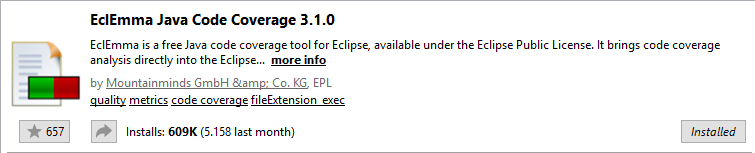
\includegraphics[scale=0.5]{EclEmma_Marketplace.png}
\caption{EclEmma im Marketplace}
\centering
\end{figure}
Zusätzlich lässt sich Jacoco auch über Maven dependencies als Plug-In einbinden. Dabei ist dann zu beachten, dass nur Jacoco eingebunden worden ist und nicht Ecl-Emma. 
\subsection{Nutzung von Ecl-Emma-Jacoco}
Nach der Installation kann EclEmma direkt „out-of-box“ genutzt werden um die Testüberdeckung zu messen oder man kann es weiter konfigurieren. So lassen sich Ordner aus der Messung exkludieren oder inkludieren. EclEmma funktioniert sowohl mit JUnit-tests als auch mit TestNG-tests und zusätzlich werden externe Testframeworks von EclEmma ebenfalls berücksichtigt. Dies wurde mit dem JavaFX UI-Testframework „testFx“ getestet. 
\bigbreak
Um die Abdeckung zu starten, muss man die Tests dann über den neuen Button in der Toolbar „Coverage“ oder „Rechtsklick \textrightarrow{} Coverage As …“ ausführen. Nachdem die Tests durchgelaufen sind, wird der Code, der getestet worden ist, farblich gekennzeichnet:rot, gelb oder grün. Rot gekennzeichnete Zeilen wurden von dem Test nicht getroffen und gelten entsprechend als nicht getestet. Gelbe Kennzeichnungen sind bedingte Anweisungen, bei dem der Test keine vollständige Abdeckung der möglichen Bedingungen bietet. Grün gekennzeichnete Zeilen sind vollständig von dem Test abgedeckt.
\begin{figure}[h]
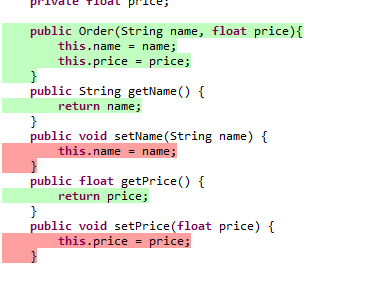
\includegraphics[scale=1.0]{Highlightning.png}
\caption{Inline Text Highlightning von Ecl-Emma}
\centering
\end{figure}
\bigbreak
Um eine bessere Übersicht für das Projekt zu haben, bietet das Plugin zusätzlich noch eine neue View an, die, wenn sie nicht bei der Installation hinzugefügt worden ist, über „Window \textrightarrow{} Show View \textrightarrow{} Other… \textrightarrow{} Coverage“ angezeigt werden lassen kann. 
\begin{figure}[h]
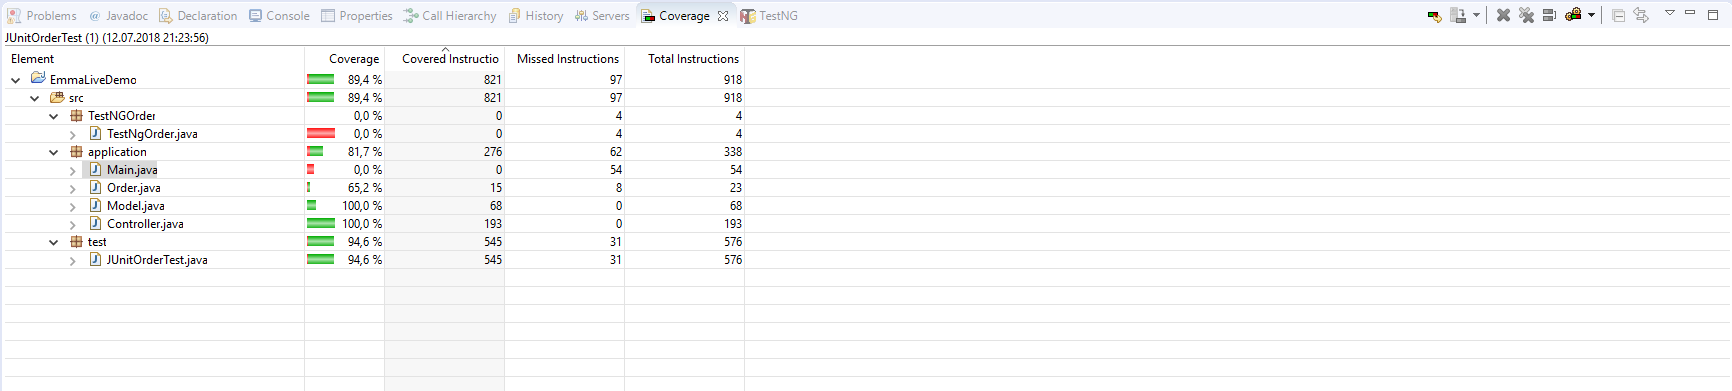
\includegraphics[scale=0.40]{Coverage_View.png}
\caption{Coverage Overview in Eclipse}
\centering
\end{figure}
\subsection{Theoretische Testabdeckung und Ecl-Emma}
In der theoretischen Testabdeckung wird zwischen verschiedenen Testabdeckungen unterschieden. Einige in der Literatur erwähnte, sind die Anweisungsüberdeckung, Zweigüberdeckung sowie die Pfadüberdeckung.~\cite{hoff}
Eine wichtige Frage ist, welche dieser Überdeckungen in der Lage ist Ecl-Emma-Jacoco zu messen? Der Dokumentation von Jacoco ist zu entnehmen, dass Jacoco in der Lage ist die Anweisungüberdeckung und die Zweigüberdeckung zu messen.~\cite{jacoco}. Daher kann mit Jacoco automatisch geprüft werden, ob die Kriterien einer zu fordernden Mindestanforderung an Qualität einer jeden Software~\cite{hoff} bei einem Java-Programm erfüllt sind.
\section{Bistro-Verwaltungs-App}
Um Ecl-Emma vorzustellen, wurde im Rahmen des Moduls eine Demo entwickelt. 
Die Demo ist eine Bistro-Verwaltungs-App, in der der Nutzer vorgegebene Menüs auswählen kann, sich einen eigenen Salat aus mehreren Rubriken zusammenstellen kann. Zusätzlich kann der Nutzer den Gesamtbetrag der Bestellung berechnen lassen, als auch Trinkgeld, in Höhe von 10\% des Gesamtbetrags, geben.
\section{Testabdeckung der Bistro-Verwaltungs-App}
Für die Demo wurden zwei Testklassen geschrieben, eine mit dem JUnit Framework, die andere mit TestNG. Beide Testklassen decken unterschiedliche Bereiche der Demo ab. 
In der JUnit Testklasse wird zusätzlich zu dem JUnit Framework noch das externe Framework „testFX“ benutzt, um UI Tests von einer JavaFX Anwendung durchzuführen.
Die jeweiligen Testklassen haben eine Testabdeckung von 53\% für den JUnit Test und eine 19,2\% Abdeckung für TestNG. 
Hierbei ist wie schon erwähnt zu beachten, dass Ecl-Emma keine Pfadüberdeckung durchführt, sondern ausschließlich Zweigabdeckung. 
\begin{figure}[h]
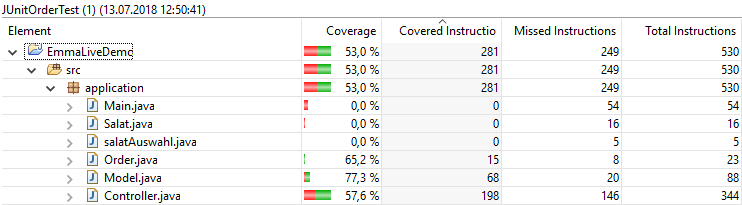
\includegraphics[scale=0.60 ]{Testabdeckung_JUnit.png}
\caption{Testabdeckung mit JUnit Tests}
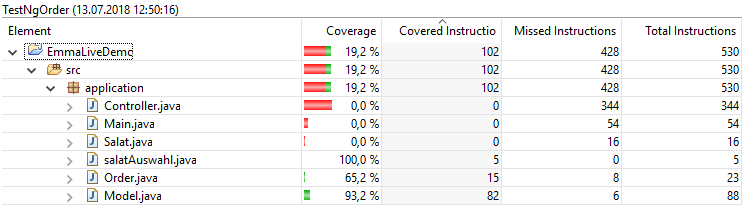
\includegraphics[scale=0.60]{Testabdeckung_TestNG.png}
\caption{Testabdeckung mit TestNG Tests}
\centering
\end{figure}

\begin{figure}[h]
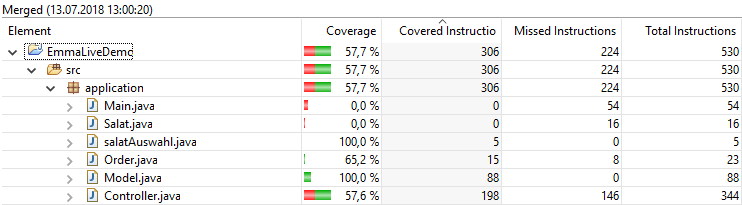
\includegraphics[scale=0.6]{Merged_Abdeckung.png}
\caption{JUnit Test Abdeckung und TestNG Abdeckung gemerged}
\centering
\end{figure}
Mit dem Ecl-Emma Plug-in lassen sich die beiden Abdeckungen mergen, um eine Übersicht über den Gesamtabdeckungsgrad der beiden Testklassen zu bekommen. Der Abdeckungsgrad des Projekts nach dem Merge durch Ecl-Emma liegt bei 57.7\%. 
\newpage
\section{Fazit}
Ecl-Emma-Jacoco ist ein Testabdeckungstool, dass sich leicht in Eclipse über den Marketplace installieren lässt. Zusätzlich ist die Bedienung des Tools sehr einfach.
Man muss zum Beispiel nicht diverse zusätzliche Java-Klassen mit ins Projekt mit einbinden. Das Tool prüft nicht die Sinnhaftigkeit von Tests, gute Testfälle zu erstellen, liegt daher weiter in den Händen des Entwicklers.
Ecl-Emma-Jacoco kann die Anweisungsüberdeckung und die Zweigüberdeckung messen. Wünschenswert wäre auch die Möglichkeit gewesen, Teile der Pfadüberdeckung messen zu können. Dadurch wäre das Tool aber sicherlich deutlich 
komplexer geworden, was dann wahrscheinlich in einer schwierigeren Bedienbarkeit resultieren würde. 
\par
Zusammengefasst ist Ecl-Emma-Jacoco ein einfaches, schnell zu installierendes Tool, was in Java-Projekten dabei helfen kann, die Testüberdeckung zu verbessern und damit auch die Qualität des gesamten Quellcodes signifikant erhöhen kann.
\begin{thebibliography}{1}
	\bibitem{hoff} \emph{Software Qualität, Dirk Hoffman} (2006)
	\bibitem{wiki} \emph{https://de.wikipedia.org/wiki/Kontrollflussorientierte\_Testverfahren} Zugriff 16.6.2018
	\bibitem{ecl-emma} \emph{https://www.jacoco.org/index.html} Zugriff 16.6.2018
	\bibitem{jacoco} \emph{https://www.jacoco.org/jacoco/trunk/doc/counters.html} Zugriff 16.6.2018
	\bibitem{code2flow} \emph{https://code2flow.com/} Zugriff 16.6.2018
\end{thebibliography}
\end{document}
